\section{Implementation of RCE-based DAQ for LBNE}


The elements of the DAQ-toolkit described in the previous section can be easily applied to the LAr TPC for LBNE.  The block diagram of a possible configuration is shown in Fig. \ref{fig:blockDiag}.  We define the "front-end DAQ" as everything between the (cold) FPGA and the ATCA shelf; from the ATCA-shelf onward is referred to as the "back-end DAQ".    The primary goal of this document is to propose a solution for the back-end DAQ and so, for this purpose, we will assume that the signals come into the back-end DAQ from the output of the front-end board (FEB) FPGA, each of which collects the output of  $8\times 16 = 128$ TPC wires.  

The basic structure of the back-end RCE-based DAQ is fairly straightforward.  The data from the ADCs is encoded (possibly using the PGP protocol; see Appendix \ref{bll}) in the FEB FPGA and driven out of the cryostat to a "flange board" which converts the electrical signal to an optical signal.  The flange board is an optional step, but one which allows the back-end DAQ crates to be conveniently placed without worrying about signal degradation.   The optical signal is then sent to the RTM which interfaces with the COB.  RTM designs with up to 48-channel fiber optic inputs exist and are currently in use by LCLS and for LSST development (???this is made up???).  The RTM also incorporates the output to the DAQ PC farm via 8 x 10 Gbps ethernet.  The RCEs on the COB can be used to perform event building or even some level of pattern recognition. 

One of the DPMs on each COB will function as the trigger and timing interface.  The  external timing and (for the 35t) trigger signals will be received via optical fiber to the RTM and will be distributed to the other DPMs and out (through the RTM) to all of the FEBs.  A scheme exists for distributing the timing and trigger over the PGP link.  

Below, we discuss some specific issues with the implementation in the 35t prototype and full LBNE, as well as some ideas for the front-end DAQ.   


%This list is just for me to organize my thoughts.
%\begin{itemize}
%\item \textbf{Data Protocol:  } Implement the PGP protocol over copper from the cold FPGA.
%\item  \textbf{Transition Board:  }  Directly after the cryostat flange (or as part of it)  convert the electrical signals to optical.  This is an optional step, but it allows us to locate the ATCA shelf anywhere without worrying about signal degradation.  Multiple signals into a single board
%\item \textbf{RTM:  } Input is 48 SNAP-12 fiber connectors based on a current (and long utilized) design.  This RTM simply converts optical to electrical and sends the data to the COB  (Is this true???).  Outputs 8 x 10 Gbps ethernet.  
%\item  \textbf{COB:  } Eight independent RCEs with PPC processors used for event building and  pattern recognition or sparsification.  Possibly use RCE FPGA to test sparsification algorithms before implementing them in the cryostat.  
%\item \textbf{ATCA Crate:  }  Provides power and communication between COBs.  Crates available in 2-, 6-, 14-slot varieties. 
%\item \textbf{Triggering:  }
%\item \textbf{Timing:  }
%\end{itemize}



\begin{figure}[p]
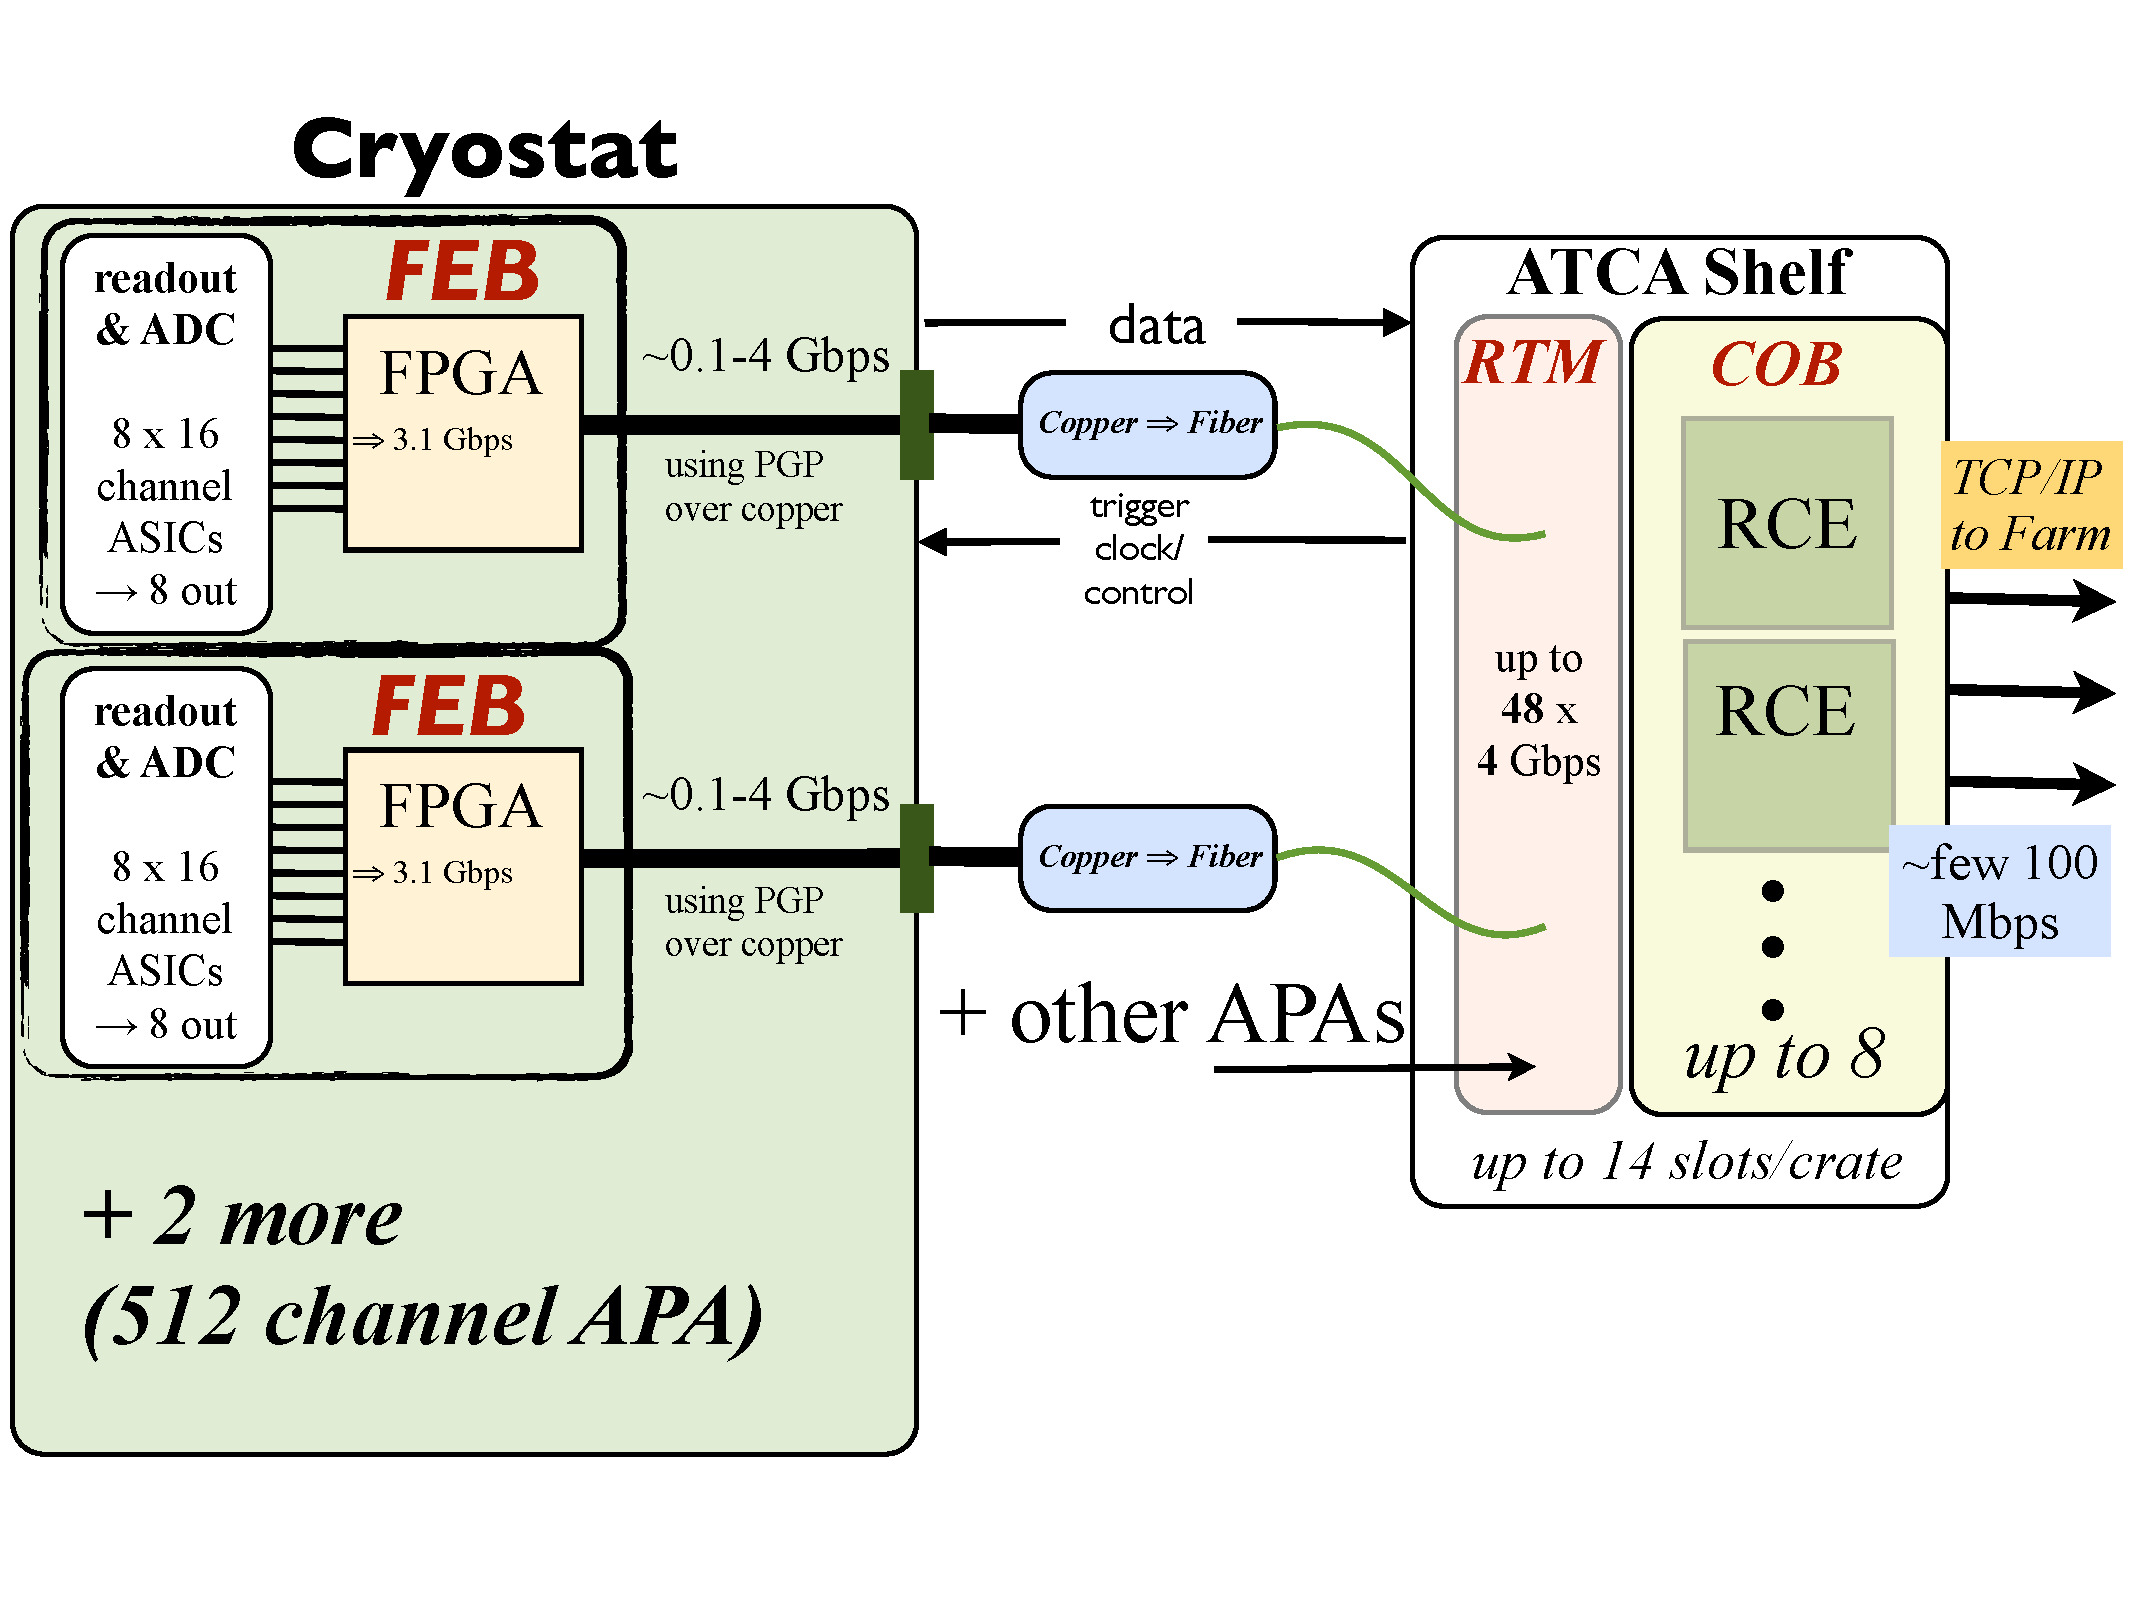
\includegraphics[scale=0.6,angle=90]{LBNE-DAQ-BlockDiagram.pdf}
\caption{Block diagram of the RCE-based DAQ for a single TPC APA.}
\label{fig:blockDiag}
\end{figure} 

\subsection{Flange Board}

The electrical signals will be brought out of the cryostat and converted to optical signals just outside the flange on custom built flange boards.   Each flange board houses optical drivers to handle the electrical-optical conversion and to transmit the optical signals to the  back-end DAQ.  The copper side of the flange board will depend on the choices made by the cold electronics group; the fiber side use SNAP-12 connectors.  The size and number of flange boards depends on the number of connections needed and mechanical specifications.  A block diagram of a two connector board is shown in Fig. \ref{fig:flange}.  Table \ref{tab:daqsumm} assumes a single pair of receiver-transmitter pairs per flange board.  



\begin{figure}[htb]
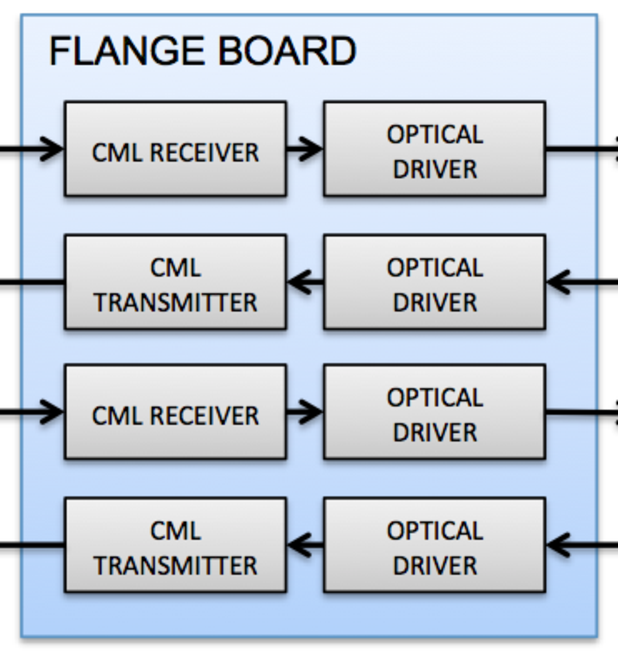
\includegraphics[scale=0.6]{flange-board.pdf}
\caption{Block diagram of a flange board with two pairs of transceivers.}
\label{fig:flange}
\end{figure} 

%================
\begin{table}[tbh]
\begin{center}
\begin{tabular}{|l|c|c|}   
\hline \hline 
    & 35t  & Full LBNE \\      
\hline
   Total Channels        & $\sim$2.3k &$\sim$307k \\ 
	Number of APAs     &  4 (?)     &    120        \\ 
   Number of FEBs       & 18 & 2400 \\ 
   Flange Boards    & 2   & 50 (assume 4 SNAP-12/board) \\ 
   RTM+COB Boards    & 1 + 1 &  50  \\
   ATCA Crates            & 1   &  4 (14-slot)   \\ 
\hline \hline
\end{tabular}
\caption[]{DAQ-related quantities for the 35t and full LBNE (as of Jan. 2013 design).  The assumption is that we will readout one wire/FEB.}
\label{tab:daqsumm} 
\end{center}
\end{table}
%=================





\subsection{DAQ Layout for 35t Prototype}

The 35t prototype TPC will have $\sim 100\times$ fewer channels than the full LBNE TPC and additionally will be externally triggered to observe cosmic rays.  The trigger rate is estimated to be  $<1$kHz.  If we run out a single wire/FEB from the cryostat, then the entire TPC can be read into a single COB.  
Bringing more wires/FEB would require more COBs; the maximum number of input channels/RTM is 48.  For 8 wires/FEB, 4 COBs are likely required, since the trigger and timing signals will take up one input to the RTM each.  

The photon system will consist of 32 digitized signals from the output of a CAEN digitizer (some of these may be sync or trigger signals).  From here, there are choices of what to do with the signals.  One option is to simply read them via the USB output into a PC and then forward that data (along with timing information) to the backend farm, bypassing the RCE-based system entirely.  Alternatively, the digitized signals could be routed to an RTM (possibly in a separate slot) and integrated with the TPC data at that stage.  This option would require some design work for the new RTM.  

In total, even if multiple wires/FEB are read out, the 35t DAQ will easily fit into a single ATCA shelf.  


%================
\begin{table}[tbh]
\begin{center}
\begin{tabular}{|l|c|c|c|}   
\hline \hline 
    											&    per-FEB               &       35t   Total   & Full LBNE  Total \\      
\hline
   Full Readout 2MHz  			  & 3.05 Gbps & 54.9 Gbps  &  7320 Gbps \\ 
   Zero-suppressed cosmics  & 15~-~?? Mbps& 270~-~?? Mbps  &  36~-~??  Gbps\\ 
  Radioactivity  ($^{39}$Ar)    & 0.6 Mbps&  11 Mbps  &   1.4 Gbps \\
   Electronics noise& 0.01 Mbps & 0.18 Mbps&  24 Mbps\\ 
\hline \hline
\end{tabular}
\caption[]{Estimated data rates per 128-channel FEB and for the entire 35t and full LBNE TPCs  (mostly from J. Urheim).}
\label{tab:datarates} 
\end{center}
\end{table}
%=================

\subsection{Full LBNE}

The basic DAQ structure for the full LBNE detector (2 $\times$ 5kT) is identical to the 35t prototype, the only difference being more channels (see Table \ref{tab:daqsumm}).  We've again assumed that we would bring out wire/FEB, although more multiplexing has been proposed in the past.  This configuration would require 50 RTM+COB pairs, which could fit in four ATCA crates; these crates could be arranged in convenient physical locations.  

The number of flange boards needed mainly depends on how many access points there are between the cryostat and the outside;  we've assumed 50 boards accepting 48-channels each (and the outputs from each flange board filling a single RTM).  This could be more or less depending on the physical layout of the cryostat.  

We have not included the photon system in this picture, as there is not sufficient detail about its layout at this point. 

\subsection{Comparision of RCE-based vs DCM-based Backend DAQ Systems}

The baseline design for the LBNE DAQ \cite{DAQ_CD1}
is based on Data Concentrator Modules (DCMs) 
that were originally designed for use in the Nova experiment.
Each of these modules takes 64 input data data streams of 20 Mbps and 
combine them into a single stream of 1 Gbps. 
The total throughput of a DCM module is limited to 60 Mbytes/second.
A single DCM module is thus able to handle enough data to readout the
entire 35 ton prototype at the expected rate of 300 Mbit/second/APA,
although without a large amount of headroom.
The main advantage of an RCE-based system is a vast improvement
in the available bandwidth, which adds signficant flexibility in 
the handling of the raw datastream.
For example, much high noise rates could be handled.
As an extreme example, one could consider reading non-zero-suppressed data 
into the DAQ system.




\subsection{High-speed Data Links From Cold FPGA to Backend DAQ}

The baseline DAQ design for the full LBNE FD envisions a high degree of zero-suppression 
occuring in the in-cryostat electronics and a rather modest total data rate (about
300 Mb/second/APA) being transmitted to the backend DAQ.
This rate would be spread over roughly 20 cables transmitting at a maximum rate of 
20 Mbit/second.
This approach has a number of advantages in that the low transmission speed is likely 
achievable with standard cables and issues of impedance matching are less of a concern.
However, it does rely on the zero-suppression algorithm being nearly perfect and has 
little headroom in case unexpected backgrounds or noise are present.

Raising the transmission bandwidth between FEB and DAQ thus seems desirable. 
An extreme case of this would be to go to the highest possible bandwidth carriable over
copper wires.
With current technology, this rate is about 5 Gbit/second. 
Cables capable of carrying this rate over distances of about 5 meters are commercially
available.

